 % Żeby nie było syfu to kolejne sekcje dodajemy do chapters/
% A potem includujemy za pomocą \input{chapters/...}

% Używamy \( \) i \[ \] zamiast dolarów -- tak jak się robi w LaTeXu


\documentclass[12pt, a4paper, polish, openany]{book}

% Please, let's familiarize ourselves with notatki.sty and tcs.sty so that we don't reinvent the wheel
\usepackage{notatki}
\DeclareMathAlphabet{\mathpzc}{OT1}{pzc}{m}{it}
\fancyhead[L]{\ensuremath{\mathbf{\mathpzc{A}}^2 \!\mid\! T \!\!\cdot\!\! L}}

\begin{document}

\begin{titlepage}

	\begin{center}
		\begin{figure}[h]
			\centering
			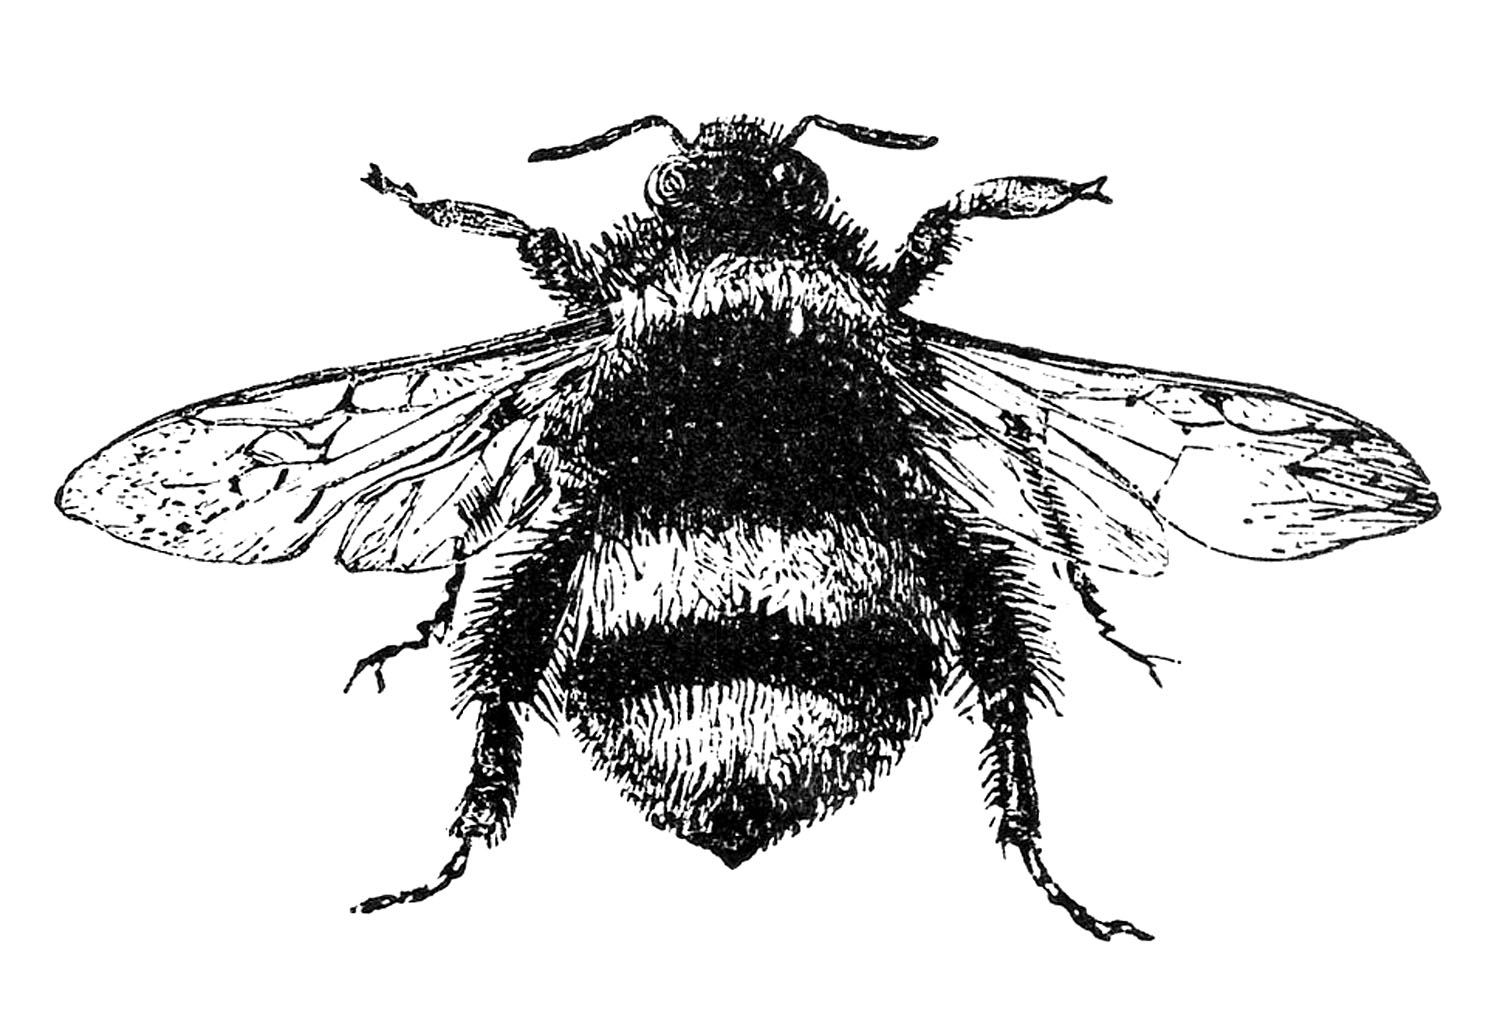
\includegraphics[scale=0.75]{img/bumblebee.jpg}
		\end{figure}
		\vspace{0.5cm}
		\Huge
		\textbf{\textsc{Metody Probabilistyczne Informatyki}}

		\vspace{0.5cm}
		\Large
		\textsc{Wybrane Dowody}

		\normalsize


		\line(1,0){330}

		\vspace{1cm}
		\textit{,,Tak teraz na to patrzę i myślę, czy ta nierówność nie powinna być w drugą stronę...''}
		\vspace{1cm}

		\textit{\textsc{Popełnione przez}}\\
		\vspace{5mm}

		\textbf{\textsc{
				Załatany Ponton \\
				V\\
				Nahtamatu\\
			}}

		\vfill

		Kraków \\
		Anno Domini 2025

	\end{center}

\end{titlepage}


\tableofcontents
\section*{Licencja}
\begin{figure}[h]
	\begin{minipage}[c]{0.25\textwidth}
		
\includegraphics[width=0.7\textwidth]{img/licencja.png}
	\end{minipage}\hfill
	\begin{minipage}[c]{0.75\textwidth}
		\caption*{
			Ten utwór jest dostępny na
			\href{https://creativecommons.org/licenses/by-sa/4.0/}{licencji Creative Commons Uznanie autorstwa
				na tych samych warunkach 4.0 Międzynarodowe.}
		}
	\end{minipage}
\end{figure}

 % Żeby nie było syfu to kolejne sekcje dodajemy do chapters/
% A potem includujemy za pomocą \input{chapters/...}

% Używamy \( \) i \[ \] zamiast dolarów -- tak jak się robi w LaTeXu


\documentclass[12pt, a4paper, polish, openany]{book}

% Please, let's familiarize ourselves with notatki.sty and tcs.sty so that we don't reinvent the wheel
\usepackage{notatki}
\fancyhead[L]{\textbf{\textit{MPI}}}

\begin{document}
% Front page and table of contents
\frontmatter

\begin{titlepage}

	\begin{center}
		\begin{figure}[h]
			\centering
			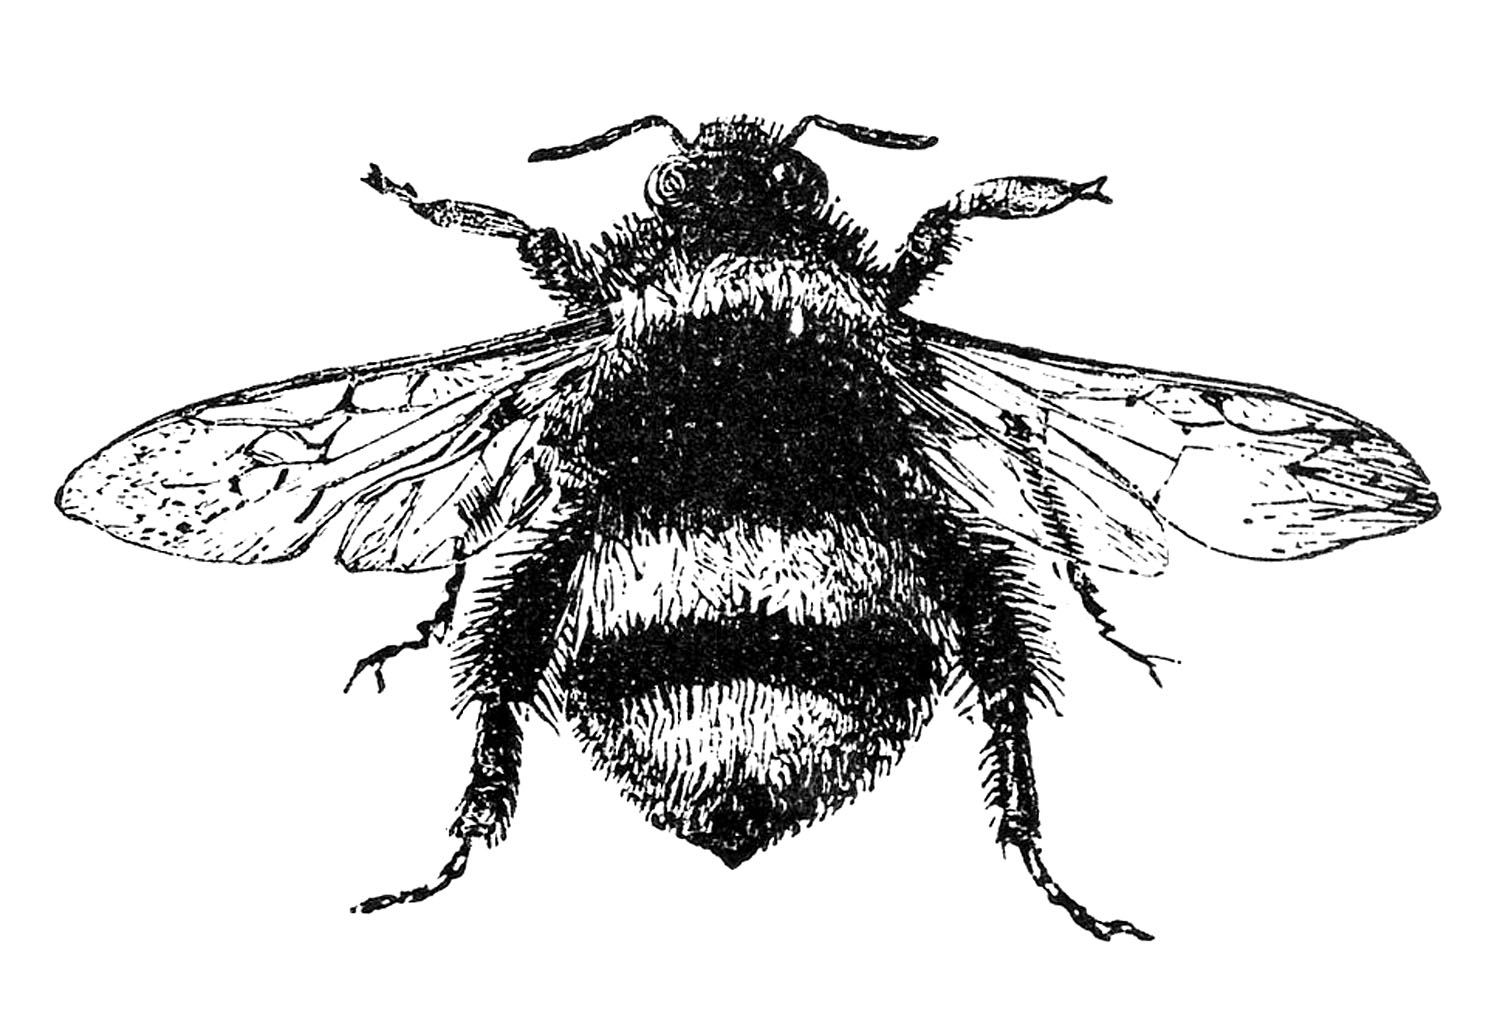
\includegraphics[scale=0.75]{img/bumblebee.jpg}
		\end{figure}
		\vspace{0.5cm}
		\Huge
		\textbf{\textsc{Metody Probabilistyczne Informatyki}}

		\vspace{0.5cm}
		\Large
		\textsc{Wybrane Dowody}

		\normalsize


		\line(1,0){330}

		\vspace{1cm}
		\textit{,,Tak teraz na to patrzę i myślę, czy ta nierówność nie powinna być w drugą stronę...''}
		\vspace{1cm}

		\textit{\textsc{Popełnione przez}}\\
		\vspace{5mm}

		\textbf{\textsc{
				Załatany Ponton \\
				V\\
				Nahtamatu\\
			}}

		\vfill

		Kraków \\
		Anno Domini 2025

	\end{center}

\end{titlepage}


\tableofcontents
\section*{Licencja}
\begin{figure}[h]
	\begin{minipage}[c]{0.25\textwidth}
		
\includegraphics[width=0.7\textwidth]{img/licencja.png}
	\end{minipage}\hfill
	\begin{minipage}[c]{0.75\textwidth}
		\caption*{
			Ten utwór jest dostępny na
			\href{https://creativecommons.org/licenses/by-sa/4.0/}{licencji Creative Commons Uznanie autorstwa
				na tych samych warunkach 4.0 Międzynarodowe.}
		}
	\end{minipage}
\end{figure}

% Remove the "Rozdział x" chapter headings, as we already number our chapters
\titleformat{\chapter}[display]{\normalfont\Huge\bfseries}{}{0pt}{\Huge}
\titlespacing*{\chapter}{0pt}{0pt}{20pt}

% Actual content
\mainmatter

\chapter{Wykład 1 (2025-10-03)}
 % Żeby nie było syfu to kolejne sekcje dodajemy do chapters/
% A potem includujemy za pomocą \input{chapters/...}

% Używamy \( \) i \[ \] zamiast dolarów -- tak jak się robi w LaTeXu


\documentclass[12pt, a4paper, polish, openany]{book}

% Please, let's familiarize ourselves with notatki.sty and tcs.sty so that we don't reinvent the wheel
\usepackage{notatki}
\fancyhead[L]{\textbf{\textit{MPI}}}

\begin{document}
% Front page and table of contents
\frontmatter

\begin{titlepage}

	\begin{center}
		\begin{figure}[h]
			\centering
			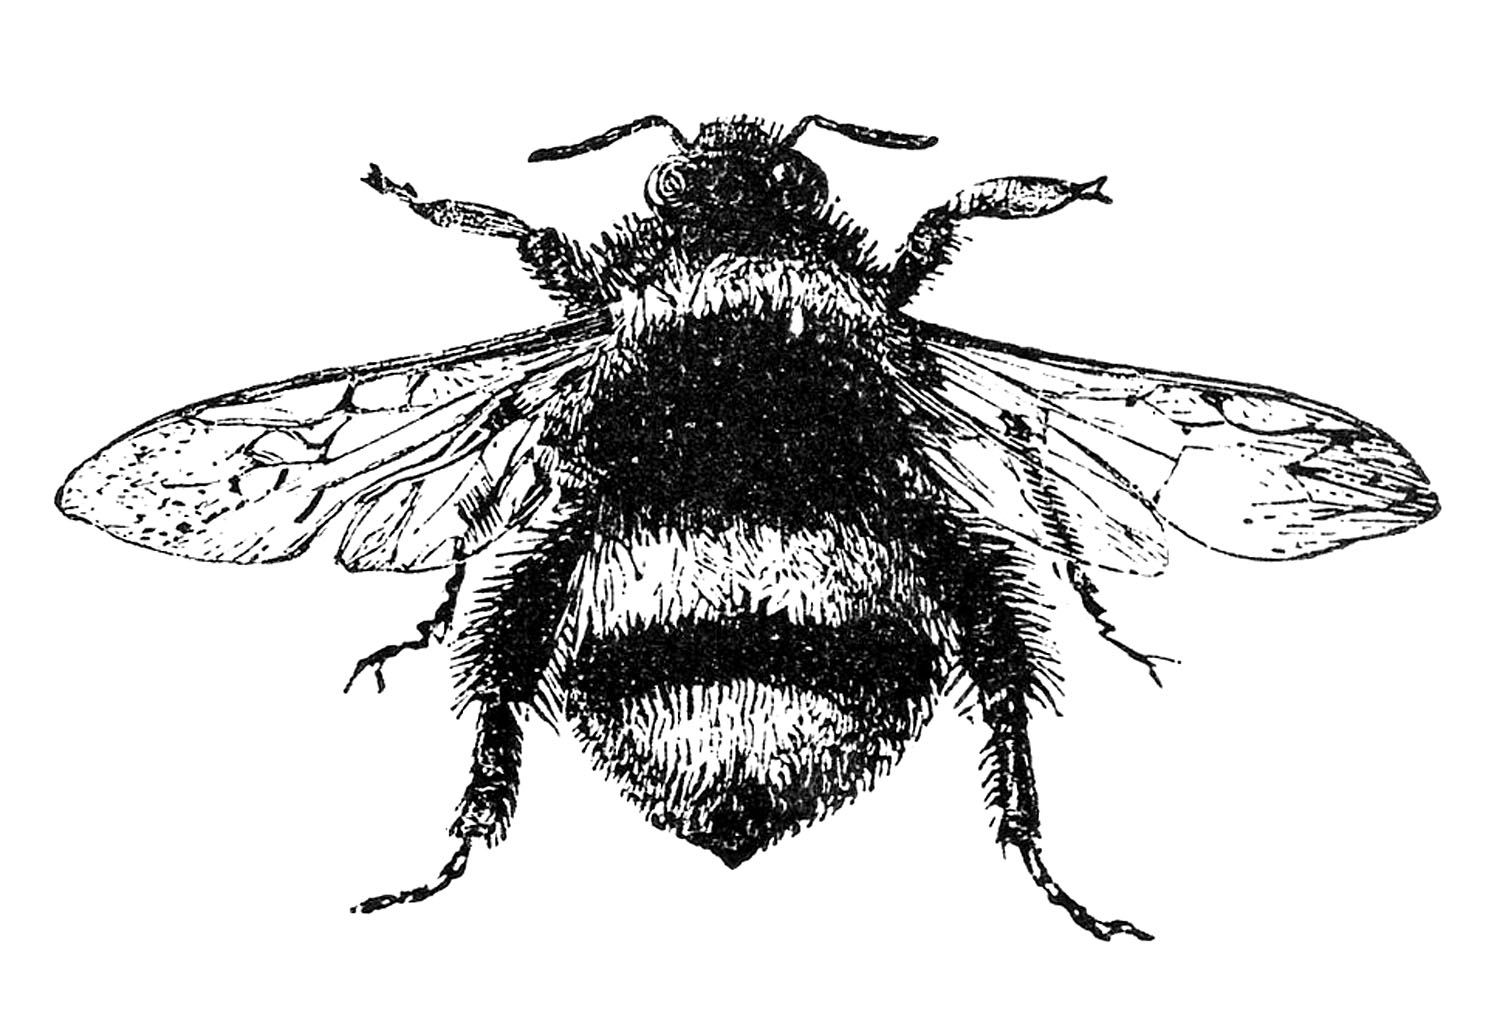
\includegraphics[scale=0.75]{img/bumblebee.jpg}
		\end{figure}
		\vspace{0.5cm}
		\Huge
		\textbf{\textsc{Metody Probabilistyczne Informatyki}}

		\vspace{0.5cm}
		\Large
		\textsc{Wybrane Dowody}

		\normalsize


		\line(1,0){330}

		\vspace{1cm}
		\textit{,,Tak teraz na to patrzę i myślę, czy ta nierówność nie powinna być w drugą stronę...''}
		\vspace{1cm}

		\textit{\textsc{Popełnione przez}}\\
		\vspace{5mm}

		\textbf{\textsc{
				Załatany Ponton \\
				V\\
				Nahtamatu\\
			}}

		\vfill

		Kraków \\
		Anno Domini 2025

	\end{center}

\end{titlepage}


\tableofcontents
\section*{Licencja}
\begin{figure}[h]
	\begin{minipage}[c]{0.25\textwidth}
		
\includegraphics[width=0.7\textwidth]{img/licencja.png}
	\end{minipage}\hfill
	\begin{minipage}[c]{0.75\textwidth}
		\caption*{
			Ten utwór jest dostępny na
			\href{https://creativecommons.org/licenses/by-sa/4.0/}{licencji Creative Commons Uznanie autorstwa
				na tych samych warunkach 4.0 Międzynarodowe.}
		}
	\end{minipage}
\end{figure}

% Remove the "Rozdział x" chapter headings, as we already number our chapters
\titleformat{\chapter}[display]{\normalfont\Huge\bfseries}{}{0pt}{\Huge}
\titlespacing*{\chapter}{0pt}{0pt}{20pt}

% Actual content
\mainmatter

\chapter{Wykład 1 (2025-10-03)}
 % Żeby nie było syfu to kolejne sekcje dodajemy do chapters/
% A potem includujemy za pomocą \input{chapters/...}

% Używamy \( \) i \[ \] zamiast dolarów -- tak jak się robi w LaTeXu


\documentclass[12pt, a4paper, polish, openany]{book}

% Please, let's familiarize ourselves with notatki.sty and tcs.sty so that we don't reinvent the wheel
\usepackage{notatki}
\fancyhead[L]{\textbf{\textit{MPI}}}

\begin{document}
% Front page and table of contents
\frontmatter

\input{titlepage}

\tableofcontents
\input{license}

% Remove the "Rozdział x" chapter headings, as we already number our chapters
\titleformat{\chapter}[display]{\normalfont\Huge\bfseries}{}{0pt}{\Huge}
\titlespacing*{\chapter}{0pt}{0pt}{20pt}

% Actual content
\mainmatter

\chapter{Wykład 1 (2025-10-03)}
\input{chapters/2025-10-03-lecture/main}

\chapter{Nagranie 1 (2025-10-04)}
\input{chapters/2025-10-04-recording/main}

\chapter{Wykład 2 (2025-10-10)}
\input{chapters/2025-10-10-lecture/main}

\chapter{Nagranie 2 (2025-10-10)}
\input{chapters/2025-10-10-recording/main}

\chapter{Wykład 3 (2025-10-17)}
\input{chapters/2025-10-17-lecture/main}

\end{document}


\chapter{Nagranie 1 (2025-10-04)}
 % Żeby nie było syfu to kolejne sekcje dodajemy do chapters/
% A potem includujemy za pomocą \input{chapters/...}

% Używamy \( \) i \[ \] zamiast dolarów -- tak jak się robi w LaTeXu


\documentclass[12pt, a4paper, polish, openany]{book}

% Please, let's familiarize ourselves with notatki.sty and tcs.sty so that we don't reinvent the wheel
\usepackage{notatki}
\fancyhead[L]{\textbf{\textit{MPI}}}

\begin{document}
% Front page and table of contents
\frontmatter

\input{titlepage}

\tableofcontents
\input{license}

% Remove the "Rozdział x" chapter headings, as we already number our chapters
\titleformat{\chapter}[display]{\normalfont\Huge\bfseries}{}{0pt}{\Huge}
\titlespacing*{\chapter}{0pt}{0pt}{20pt}

% Actual content
\mainmatter

\chapter{Wykład 1 (2025-10-03)}
\input{chapters/2025-10-03-lecture/main}

\chapter{Nagranie 1 (2025-10-04)}
\input{chapters/2025-10-04-recording/main}

\chapter{Wykład 2 (2025-10-10)}
\input{chapters/2025-10-10-lecture/main}

\chapter{Nagranie 2 (2025-10-10)}
\input{chapters/2025-10-10-recording/main}

\chapter{Wykład 3 (2025-10-17)}
\input{chapters/2025-10-17-lecture/main}

\end{document}


\chapter{Wykład 2 (2025-10-10)}
 % Żeby nie było syfu to kolejne sekcje dodajemy do chapters/
% A potem includujemy za pomocą \input{chapters/...}

% Używamy \( \) i \[ \] zamiast dolarów -- tak jak się robi w LaTeXu


\documentclass[12pt, a4paper, polish, openany]{book}

% Please, let's familiarize ourselves with notatki.sty and tcs.sty so that we don't reinvent the wheel
\usepackage{notatki}
\fancyhead[L]{\textbf{\textit{MPI}}}

\begin{document}
% Front page and table of contents
\frontmatter

\input{titlepage}

\tableofcontents
\input{license}

% Remove the "Rozdział x" chapter headings, as we already number our chapters
\titleformat{\chapter}[display]{\normalfont\Huge\bfseries}{}{0pt}{\Huge}
\titlespacing*{\chapter}{0pt}{0pt}{20pt}

% Actual content
\mainmatter

\chapter{Wykład 1 (2025-10-03)}
\input{chapters/2025-10-03-lecture/main}

\chapter{Nagranie 1 (2025-10-04)}
\input{chapters/2025-10-04-recording/main}

\chapter{Wykład 2 (2025-10-10)}
\input{chapters/2025-10-10-lecture/main}

\chapter{Nagranie 2 (2025-10-10)}
\input{chapters/2025-10-10-recording/main}

\chapter{Wykład 3 (2025-10-17)}
\input{chapters/2025-10-17-lecture/main}

\end{document}


\chapter{Nagranie 2 (2025-10-10)}
 % Żeby nie było syfu to kolejne sekcje dodajemy do chapters/
% A potem includujemy za pomocą \input{chapters/...}

% Używamy \( \) i \[ \] zamiast dolarów -- tak jak się robi w LaTeXu


\documentclass[12pt, a4paper, polish, openany]{book}

% Please, let's familiarize ourselves with notatki.sty and tcs.sty so that we don't reinvent the wheel
\usepackage{notatki}
\fancyhead[L]{\textbf{\textit{MPI}}}

\begin{document}
% Front page and table of contents
\frontmatter

\input{titlepage}

\tableofcontents
\input{license}

% Remove the "Rozdział x" chapter headings, as we already number our chapters
\titleformat{\chapter}[display]{\normalfont\Huge\bfseries}{}{0pt}{\Huge}
\titlespacing*{\chapter}{0pt}{0pt}{20pt}

% Actual content
\mainmatter

\chapter{Wykład 1 (2025-10-03)}
\input{chapters/2025-10-03-lecture/main}

\chapter{Nagranie 1 (2025-10-04)}
\input{chapters/2025-10-04-recording/main}

\chapter{Wykład 2 (2025-10-10)}
\input{chapters/2025-10-10-lecture/main}

\chapter{Nagranie 2 (2025-10-10)}
\input{chapters/2025-10-10-recording/main}

\chapter{Wykład 3 (2025-10-17)}
\input{chapters/2025-10-17-lecture/main}

\end{document}


\chapter{Wykład 3 (2025-10-17)}
 % Żeby nie było syfu to kolejne sekcje dodajemy do chapters/
% A potem includujemy za pomocą \input{chapters/...}

% Używamy \( \) i \[ \] zamiast dolarów -- tak jak się robi w LaTeXu


\documentclass[12pt, a4paper, polish, openany]{book}

% Please, let's familiarize ourselves with notatki.sty and tcs.sty so that we don't reinvent the wheel
\usepackage{notatki}
\fancyhead[L]{\textbf{\textit{MPI}}}

\begin{document}
% Front page and table of contents
\frontmatter

\input{titlepage}

\tableofcontents
\input{license}

% Remove the "Rozdział x" chapter headings, as we already number our chapters
\titleformat{\chapter}[display]{\normalfont\Huge\bfseries}{}{0pt}{\Huge}
\titlespacing*{\chapter}{0pt}{0pt}{20pt}

% Actual content
\mainmatter

\chapter{Wykład 1 (2025-10-03)}
\input{chapters/2025-10-03-lecture/main}

\chapter{Nagranie 1 (2025-10-04)}
\input{chapters/2025-10-04-recording/main}

\chapter{Wykład 2 (2025-10-10)}
\input{chapters/2025-10-10-lecture/main}

\chapter{Nagranie 2 (2025-10-10)}
\input{chapters/2025-10-10-recording/main}

\chapter{Wykład 3 (2025-10-17)}
\input{chapters/2025-10-17-lecture/main}

\end{document}


\end{document}


\chapter{Nagranie 1 (2025-10-04)}
 % Żeby nie było syfu to kolejne sekcje dodajemy do chapters/
% A potem includujemy za pomocą \input{chapters/...}

% Używamy \( \) i \[ \] zamiast dolarów -- tak jak się robi w LaTeXu


\documentclass[12pt, a4paper, polish, openany]{book}

% Please, let's familiarize ourselves with notatki.sty and tcs.sty so that we don't reinvent the wheel
\usepackage{notatki}
\fancyhead[L]{\textbf{\textit{MPI}}}

\begin{document}
% Front page and table of contents
\frontmatter

\begin{titlepage}

	\begin{center}
		\begin{figure}[h]
			\centering
			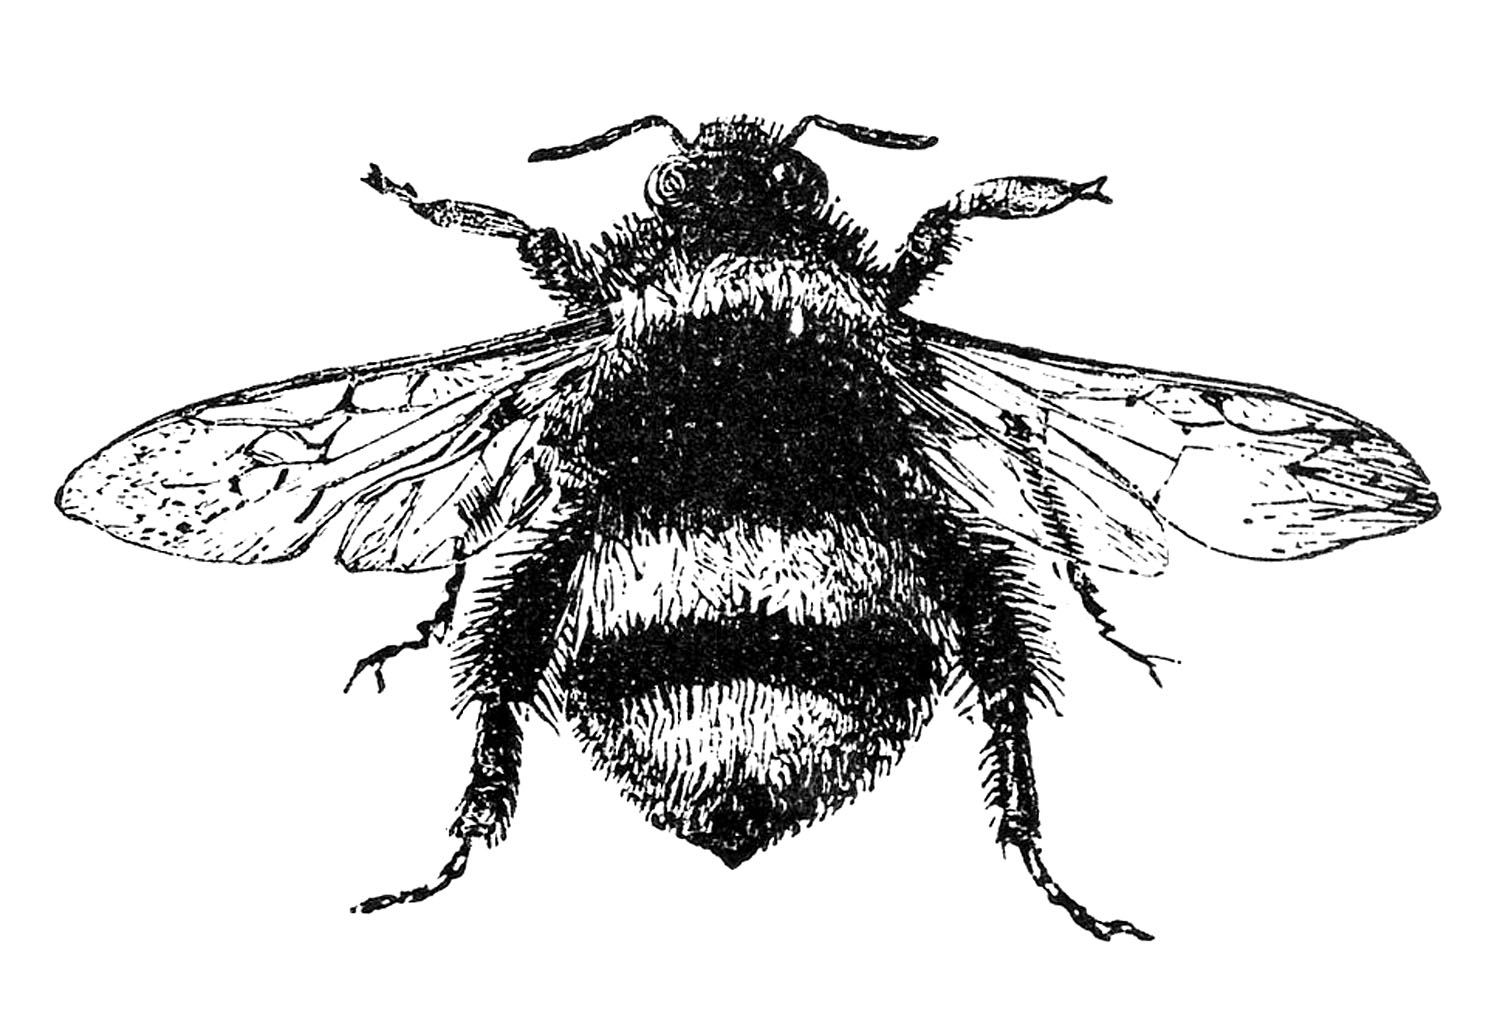
\includegraphics[scale=0.75]{img/bumblebee.jpg}
		\end{figure}
		\vspace{0.5cm}
		\Huge
		\textbf{\textsc{Metody Probabilistyczne Informatyki}}

		\vspace{0.5cm}
		\Large
		\textsc{Wybrane Dowody}

		\normalsize


		\line(1,0){330}

		\vspace{1cm}
		\textit{,,Tak teraz na to patrzę i myślę, czy ta nierówność nie powinna być w drugą stronę...''}
		\vspace{1cm}

		\textit{\textsc{Popełnione przez}}\\
		\vspace{5mm}

		\textbf{\textsc{
				Załatany Ponton \\
				V\\
				Nahtamatu\\
			}}

		\vfill

		Kraków \\
		Anno Domini 2025

	\end{center}

\end{titlepage}


\tableofcontents
\section*{Licencja}
\begin{figure}[h]
	\begin{minipage}[c]{0.25\textwidth}
		
\includegraphics[width=0.7\textwidth]{img/licencja.png}
	\end{minipage}\hfill
	\begin{minipage}[c]{0.75\textwidth}
		\caption*{
			Ten utwór jest dostępny na
			\href{https://creativecommons.org/licenses/by-sa/4.0/}{licencji Creative Commons Uznanie autorstwa
				na tych samych warunkach 4.0 Międzynarodowe.}
		}
	\end{minipage}
\end{figure}

% Remove the "Rozdział x" chapter headings, as we already number our chapters
\titleformat{\chapter}[display]{\normalfont\Huge\bfseries}{}{0pt}{\Huge}
\titlespacing*{\chapter}{0pt}{0pt}{20pt}

% Actual content
\mainmatter

\chapter{Wykład 1 (2025-10-03)}
 % Żeby nie było syfu to kolejne sekcje dodajemy do chapters/
% A potem includujemy za pomocą \input{chapters/...}

% Używamy \( \) i \[ \] zamiast dolarów -- tak jak się robi w LaTeXu


\documentclass[12pt, a4paper, polish, openany]{book}

% Please, let's familiarize ourselves with notatki.sty and tcs.sty so that we don't reinvent the wheel
\usepackage{notatki}
\fancyhead[L]{\textbf{\textit{MPI}}}

\begin{document}
% Front page and table of contents
\frontmatter

\input{titlepage}

\tableofcontents
\input{license}

% Remove the "Rozdział x" chapter headings, as we already number our chapters
\titleformat{\chapter}[display]{\normalfont\Huge\bfseries}{}{0pt}{\Huge}
\titlespacing*{\chapter}{0pt}{0pt}{20pt}

% Actual content
\mainmatter

\chapter{Wykład 1 (2025-10-03)}
\input{chapters/2025-10-03-lecture/main}

\chapter{Nagranie 1 (2025-10-04)}
\input{chapters/2025-10-04-recording/main}

\chapter{Wykład 2 (2025-10-10)}
\input{chapters/2025-10-10-lecture/main}

\chapter{Nagranie 2 (2025-10-10)}
\input{chapters/2025-10-10-recording/main}

\chapter{Wykład 3 (2025-10-17)}
\input{chapters/2025-10-17-lecture/main}

\end{document}


\chapter{Nagranie 1 (2025-10-04)}
 % Żeby nie było syfu to kolejne sekcje dodajemy do chapters/
% A potem includujemy za pomocą \input{chapters/...}

% Używamy \( \) i \[ \] zamiast dolarów -- tak jak się robi w LaTeXu


\documentclass[12pt, a4paper, polish, openany]{book}

% Please, let's familiarize ourselves with notatki.sty and tcs.sty so that we don't reinvent the wheel
\usepackage{notatki}
\fancyhead[L]{\textbf{\textit{MPI}}}

\begin{document}
% Front page and table of contents
\frontmatter

\input{titlepage}

\tableofcontents
\input{license}

% Remove the "Rozdział x" chapter headings, as we already number our chapters
\titleformat{\chapter}[display]{\normalfont\Huge\bfseries}{}{0pt}{\Huge}
\titlespacing*{\chapter}{0pt}{0pt}{20pt}

% Actual content
\mainmatter

\chapter{Wykład 1 (2025-10-03)}
\input{chapters/2025-10-03-lecture/main}

\chapter{Nagranie 1 (2025-10-04)}
\input{chapters/2025-10-04-recording/main}

\chapter{Wykład 2 (2025-10-10)}
\input{chapters/2025-10-10-lecture/main}

\chapter{Nagranie 2 (2025-10-10)}
\input{chapters/2025-10-10-recording/main}

\chapter{Wykład 3 (2025-10-17)}
\input{chapters/2025-10-17-lecture/main}

\end{document}


\chapter{Wykład 2 (2025-10-10)}
 % Żeby nie było syfu to kolejne sekcje dodajemy do chapters/
% A potem includujemy za pomocą \input{chapters/...}

% Używamy \( \) i \[ \] zamiast dolarów -- tak jak się robi w LaTeXu


\documentclass[12pt, a4paper, polish, openany]{book}

% Please, let's familiarize ourselves with notatki.sty and tcs.sty so that we don't reinvent the wheel
\usepackage{notatki}
\fancyhead[L]{\textbf{\textit{MPI}}}

\begin{document}
% Front page and table of contents
\frontmatter

\input{titlepage}

\tableofcontents
\input{license}

% Remove the "Rozdział x" chapter headings, as we already number our chapters
\titleformat{\chapter}[display]{\normalfont\Huge\bfseries}{}{0pt}{\Huge}
\titlespacing*{\chapter}{0pt}{0pt}{20pt}

% Actual content
\mainmatter

\chapter{Wykład 1 (2025-10-03)}
\input{chapters/2025-10-03-lecture/main}

\chapter{Nagranie 1 (2025-10-04)}
\input{chapters/2025-10-04-recording/main}

\chapter{Wykład 2 (2025-10-10)}
\input{chapters/2025-10-10-lecture/main}

\chapter{Nagranie 2 (2025-10-10)}
\input{chapters/2025-10-10-recording/main}

\chapter{Wykład 3 (2025-10-17)}
\input{chapters/2025-10-17-lecture/main}

\end{document}


\chapter{Nagranie 2 (2025-10-10)}
 % Żeby nie było syfu to kolejne sekcje dodajemy do chapters/
% A potem includujemy za pomocą \input{chapters/...}

% Używamy \( \) i \[ \] zamiast dolarów -- tak jak się robi w LaTeXu


\documentclass[12pt, a4paper, polish, openany]{book}

% Please, let's familiarize ourselves with notatki.sty and tcs.sty so that we don't reinvent the wheel
\usepackage{notatki}
\fancyhead[L]{\textbf{\textit{MPI}}}

\begin{document}
% Front page and table of contents
\frontmatter

\input{titlepage}

\tableofcontents
\input{license}

% Remove the "Rozdział x" chapter headings, as we already number our chapters
\titleformat{\chapter}[display]{\normalfont\Huge\bfseries}{}{0pt}{\Huge}
\titlespacing*{\chapter}{0pt}{0pt}{20pt}

% Actual content
\mainmatter

\chapter{Wykład 1 (2025-10-03)}
\input{chapters/2025-10-03-lecture/main}

\chapter{Nagranie 1 (2025-10-04)}
\input{chapters/2025-10-04-recording/main}

\chapter{Wykład 2 (2025-10-10)}
\input{chapters/2025-10-10-lecture/main}

\chapter{Nagranie 2 (2025-10-10)}
\input{chapters/2025-10-10-recording/main}

\chapter{Wykład 3 (2025-10-17)}
\input{chapters/2025-10-17-lecture/main}

\end{document}


\chapter{Wykład 3 (2025-10-17)}
 % Żeby nie było syfu to kolejne sekcje dodajemy do chapters/
% A potem includujemy za pomocą \input{chapters/...}

% Używamy \( \) i \[ \] zamiast dolarów -- tak jak się robi w LaTeXu


\documentclass[12pt, a4paper, polish, openany]{book}

% Please, let's familiarize ourselves with notatki.sty and tcs.sty so that we don't reinvent the wheel
\usepackage{notatki}
\fancyhead[L]{\textbf{\textit{MPI}}}

\begin{document}
% Front page and table of contents
\frontmatter

\input{titlepage}

\tableofcontents
\input{license}

% Remove the "Rozdział x" chapter headings, as we already number our chapters
\titleformat{\chapter}[display]{\normalfont\Huge\bfseries}{}{0pt}{\Huge}
\titlespacing*{\chapter}{0pt}{0pt}{20pt}

% Actual content
\mainmatter

\chapter{Wykład 1 (2025-10-03)}
\input{chapters/2025-10-03-lecture/main}

\chapter{Nagranie 1 (2025-10-04)}
\input{chapters/2025-10-04-recording/main}

\chapter{Wykład 2 (2025-10-10)}
\input{chapters/2025-10-10-lecture/main}

\chapter{Nagranie 2 (2025-10-10)}
\input{chapters/2025-10-10-recording/main}

\chapter{Wykład 3 (2025-10-17)}
\input{chapters/2025-10-17-lecture/main}

\end{document}


\end{document}


\chapter{Wykład 2 (2025-10-10)}
 % Żeby nie było syfu to kolejne sekcje dodajemy do chapters/
% A potem includujemy za pomocą \input{chapters/...}

% Używamy \( \) i \[ \] zamiast dolarów -- tak jak się robi w LaTeXu


\documentclass[12pt, a4paper, polish, openany]{book}

% Please, let's familiarize ourselves with notatki.sty and tcs.sty so that we don't reinvent the wheel
\usepackage{notatki}
\fancyhead[L]{\textbf{\textit{MPI}}}

\begin{document}
% Front page and table of contents
\frontmatter

\begin{titlepage}

	\begin{center}
		\begin{figure}[h]
			\centering
			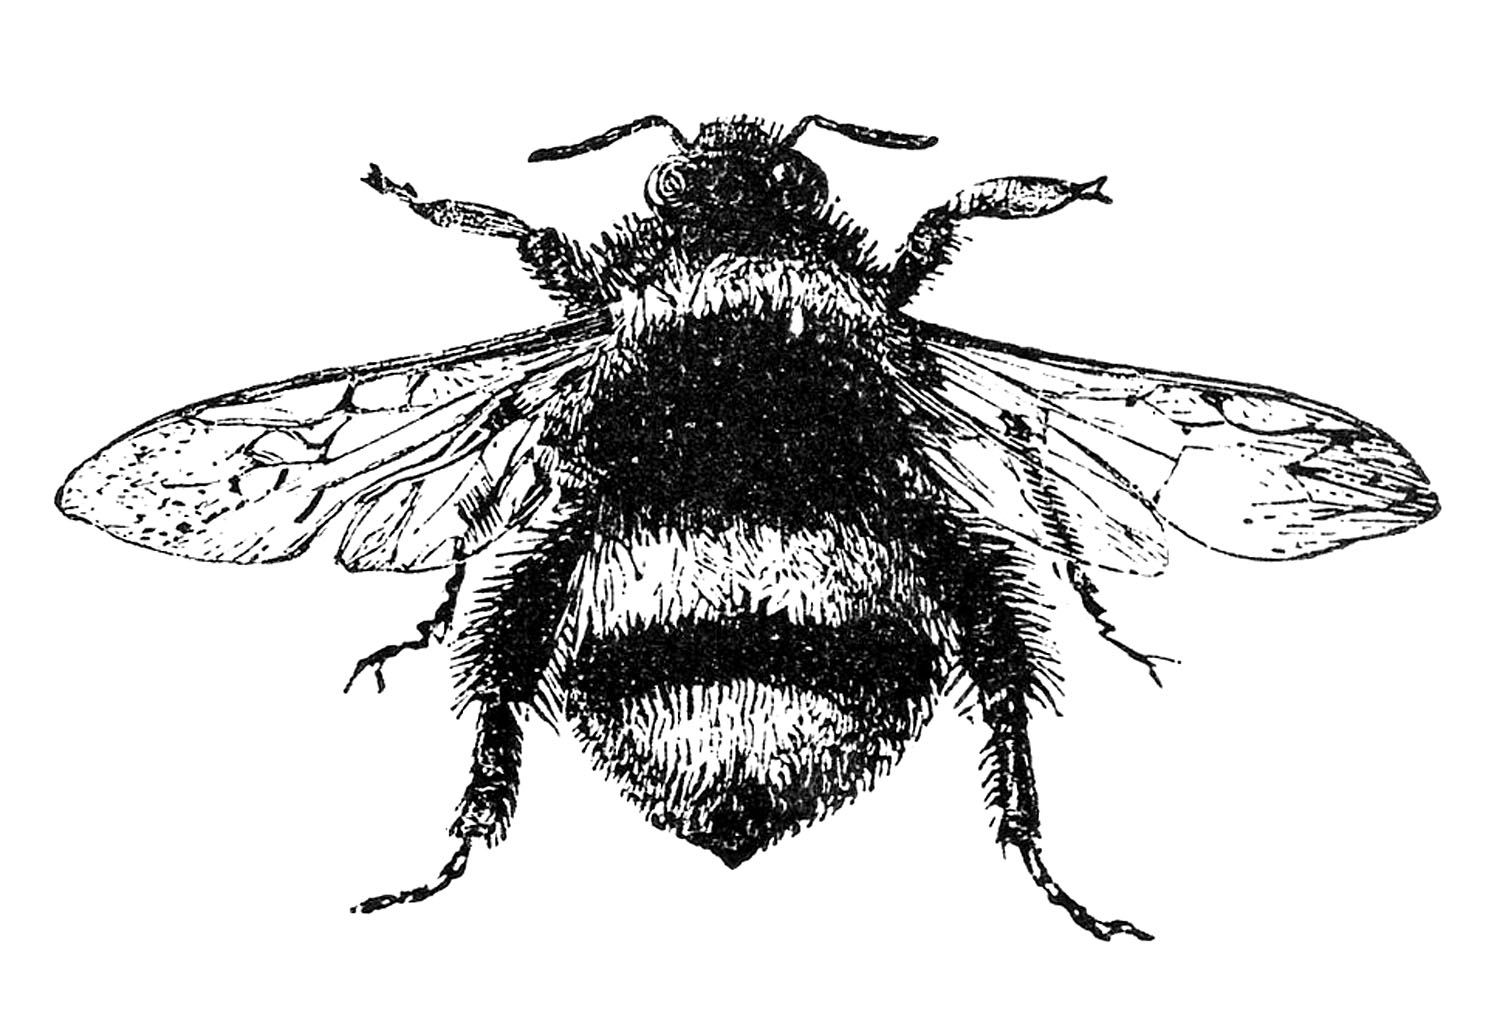
\includegraphics[scale=0.75]{img/bumblebee.jpg}
		\end{figure}
		\vspace{0.5cm}
		\Huge
		\textbf{\textsc{Metody Probabilistyczne Informatyki}}

		\vspace{0.5cm}
		\Large
		\textsc{Wybrane Dowody}

		\normalsize


		\line(1,0){330}

		\vspace{1cm}
		\textit{,,Tak teraz na to patrzę i myślę, czy ta nierówność nie powinna być w drugą stronę...''}
		\vspace{1cm}

		\textit{\textsc{Popełnione przez}}\\
		\vspace{5mm}

		\textbf{\textsc{
				Załatany Ponton \\
				V\\
				Nahtamatu\\
			}}

		\vfill

		Kraków \\
		Anno Domini 2025

	\end{center}

\end{titlepage}


\tableofcontents
\section*{Licencja}
\begin{figure}[h]
	\begin{minipage}[c]{0.25\textwidth}
		
\includegraphics[width=0.7\textwidth]{img/licencja.png}
	\end{minipage}\hfill
	\begin{minipage}[c]{0.75\textwidth}
		\caption*{
			Ten utwór jest dostępny na
			\href{https://creativecommons.org/licenses/by-sa/4.0/}{licencji Creative Commons Uznanie autorstwa
				na tych samych warunkach 4.0 Międzynarodowe.}
		}
	\end{minipage}
\end{figure}

% Remove the "Rozdział x" chapter headings, as we already number our chapters
\titleformat{\chapter}[display]{\normalfont\Huge\bfseries}{}{0pt}{\Huge}
\titlespacing*{\chapter}{0pt}{0pt}{20pt}

% Actual content
\mainmatter

\chapter{Wykład 1 (2025-10-03)}
 % Żeby nie było syfu to kolejne sekcje dodajemy do chapters/
% A potem includujemy za pomocą \input{chapters/...}

% Używamy \( \) i \[ \] zamiast dolarów -- tak jak się robi w LaTeXu


\documentclass[12pt, a4paper, polish, openany]{book}

% Please, let's familiarize ourselves with notatki.sty and tcs.sty so that we don't reinvent the wheel
\usepackage{notatki}
\fancyhead[L]{\textbf{\textit{MPI}}}

\begin{document}
% Front page and table of contents
\frontmatter

\input{titlepage}

\tableofcontents
\input{license}

% Remove the "Rozdział x" chapter headings, as we already number our chapters
\titleformat{\chapter}[display]{\normalfont\Huge\bfseries}{}{0pt}{\Huge}
\titlespacing*{\chapter}{0pt}{0pt}{20pt}

% Actual content
\mainmatter

\chapter{Wykład 1 (2025-10-03)}
\input{chapters/2025-10-03-lecture/main}

\chapter{Nagranie 1 (2025-10-04)}
\input{chapters/2025-10-04-recording/main}

\chapter{Wykład 2 (2025-10-10)}
\input{chapters/2025-10-10-lecture/main}

\chapter{Nagranie 2 (2025-10-10)}
\input{chapters/2025-10-10-recording/main}

\chapter{Wykład 3 (2025-10-17)}
\input{chapters/2025-10-17-lecture/main}

\end{document}


\chapter{Nagranie 1 (2025-10-04)}
 % Żeby nie było syfu to kolejne sekcje dodajemy do chapters/
% A potem includujemy za pomocą \input{chapters/...}

% Używamy \( \) i \[ \] zamiast dolarów -- tak jak się robi w LaTeXu


\documentclass[12pt, a4paper, polish, openany]{book}

% Please, let's familiarize ourselves with notatki.sty and tcs.sty so that we don't reinvent the wheel
\usepackage{notatki}
\fancyhead[L]{\textbf{\textit{MPI}}}

\begin{document}
% Front page and table of contents
\frontmatter

\input{titlepage}

\tableofcontents
\input{license}

% Remove the "Rozdział x" chapter headings, as we already number our chapters
\titleformat{\chapter}[display]{\normalfont\Huge\bfseries}{}{0pt}{\Huge}
\titlespacing*{\chapter}{0pt}{0pt}{20pt}

% Actual content
\mainmatter

\chapter{Wykład 1 (2025-10-03)}
\input{chapters/2025-10-03-lecture/main}

\chapter{Nagranie 1 (2025-10-04)}
\input{chapters/2025-10-04-recording/main}

\chapter{Wykład 2 (2025-10-10)}
\input{chapters/2025-10-10-lecture/main}

\chapter{Nagranie 2 (2025-10-10)}
\input{chapters/2025-10-10-recording/main}

\chapter{Wykład 3 (2025-10-17)}
\input{chapters/2025-10-17-lecture/main}

\end{document}


\chapter{Wykład 2 (2025-10-10)}
 % Żeby nie było syfu to kolejne sekcje dodajemy do chapters/
% A potem includujemy za pomocą \input{chapters/...}

% Używamy \( \) i \[ \] zamiast dolarów -- tak jak się robi w LaTeXu


\documentclass[12pt, a4paper, polish, openany]{book}

% Please, let's familiarize ourselves with notatki.sty and tcs.sty so that we don't reinvent the wheel
\usepackage{notatki}
\fancyhead[L]{\textbf{\textit{MPI}}}

\begin{document}
% Front page and table of contents
\frontmatter

\input{titlepage}

\tableofcontents
\input{license}

% Remove the "Rozdział x" chapter headings, as we already number our chapters
\titleformat{\chapter}[display]{\normalfont\Huge\bfseries}{}{0pt}{\Huge}
\titlespacing*{\chapter}{0pt}{0pt}{20pt}

% Actual content
\mainmatter

\chapter{Wykład 1 (2025-10-03)}
\input{chapters/2025-10-03-lecture/main}

\chapter{Nagranie 1 (2025-10-04)}
\input{chapters/2025-10-04-recording/main}

\chapter{Wykład 2 (2025-10-10)}
\input{chapters/2025-10-10-lecture/main}

\chapter{Nagranie 2 (2025-10-10)}
\input{chapters/2025-10-10-recording/main}

\chapter{Wykład 3 (2025-10-17)}
\input{chapters/2025-10-17-lecture/main}

\end{document}


\chapter{Nagranie 2 (2025-10-10)}
 % Żeby nie było syfu to kolejne sekcje dodajemy do chapters/
% A potem includujemy za pomocą \input{chapters/...}

% Używamy \( \) i \[ \] zamiast dolarów -- tak jak się robi w LaTeXu


\documentclass[12pt, a4paper, polish, openany]{book}

% Please, let's familiarize ourselves with notatki.sty and tcs.sty so that we don't reinvent the wheel
\usepackage{notatki}
\fancyhead[L]{\textbf{\textit{MPI}}}

\begin{document}
% Front page and table of contents
\frontmatter

\input{titlepage}

\tableofcontents
\input{license}

% Remove the "Rozdział x" chapter headings, as we already number our chapters
\titleformat{\chapter}[display]{\normalfont\Huge\bfseries}{}{0pt}{\Huge}
\titlespacing*{\chapter}{0pt}{0pt}{20pt}

% Actual content
\mainmatter

\chapter{Wykład 1 (2025-10-03)}
\input{chapters/2025-10-03-lecture/main}

\chapter{Nagranie 1 (2025-10-04)}
\input{chapters/2025-10-04-recording/main}

\chapter{Wykład 2 (2025-10-10)}
\input{chapters/2025-10-10-lecture/main}

\chapter{Nagranie 2 (2025-10-10)}
\input{chapters/2025-10-10-recording/main}

\chapter{Wykład 3 (2025-10-17)}
\input{chapters/2025-10-17-lecture/main}

\end{document}


\chapter{Wykład 3 (2025-10-17)}
 % Żeby nie było syfu to kolejne sekcje dodajemy do chapters/
% A potem includujemy za pomocą \input{chapters/...}

% Używamy \( \) i \[ \] zamiast dolarów -- tak jak się robi w LaTeXu


\documentclass[12pt, a4paper, polish, openany]{book}

% Please, let's familiarize ourselves with notatki.sty and tcs.sty so that we don't reinvent the wheel
\usepackage{notatki}
\fancyhead[L]{\textbf{\textit{MPI}}}

\begin{document}
% Front page and table of contents
\frontmatter

\input{titlepage}

\tableofcontents
\input{license}

% Remove the "Rozdział x" chapter headings, as we already number our chapters
\titleformat{\chapter}[display]{\normalfont\Huge\bfseries}{}{0pt}{\Huge}
\titlespacing*{\chapter}{0pt}{0pt}{20pt}

% Actual content
\mainmatter

\chapter{Wykład 1 (2025-10-03)}
\input{chapters/2025-10-03-lecture/main}

\chapter{Nagranie 1 (2025-10-04)}
\input{chapters/2025-10-04-recording/main}

\chapter{Wykład 2 (2025-10-10)}
\input{chapters/2025-10-10-lecture/main}

\chapter{Nagranie 2 (2025-10-10)}
\input{chapters/2025-10-10-recording/main}

\chapter{Wykład 3 (2025-10-17)}
\input{chapters/2025-10-17-lecture/main}

\end{document}


\end{document}


\chapter{Nagranie 2 (2025-10-10)}
 % Żeby nie było syfu to kolejne sekcje dodajemy do chapters/
% A potem includujemy za pomocą \input{chapters/...}

% Używamy \( \) i \[ \] zamiast dolarów -- tak jak się robi w LaTeXu


\documentclass[12pt, a4paper, polish, openany]{book}

% Please, let's familiarize ourselves with notatki.sty and tcs.sty so that we don't reinvent the wheel
\usepackage{notatki}
\fancyhead[L]{\textbf{\textit{MPI}}}

\begin{document}
% Front page and table of contents
\frontmatter

\begin{titlepage}

	\begin{center}
		\begin{figure}[h]
			\centering
			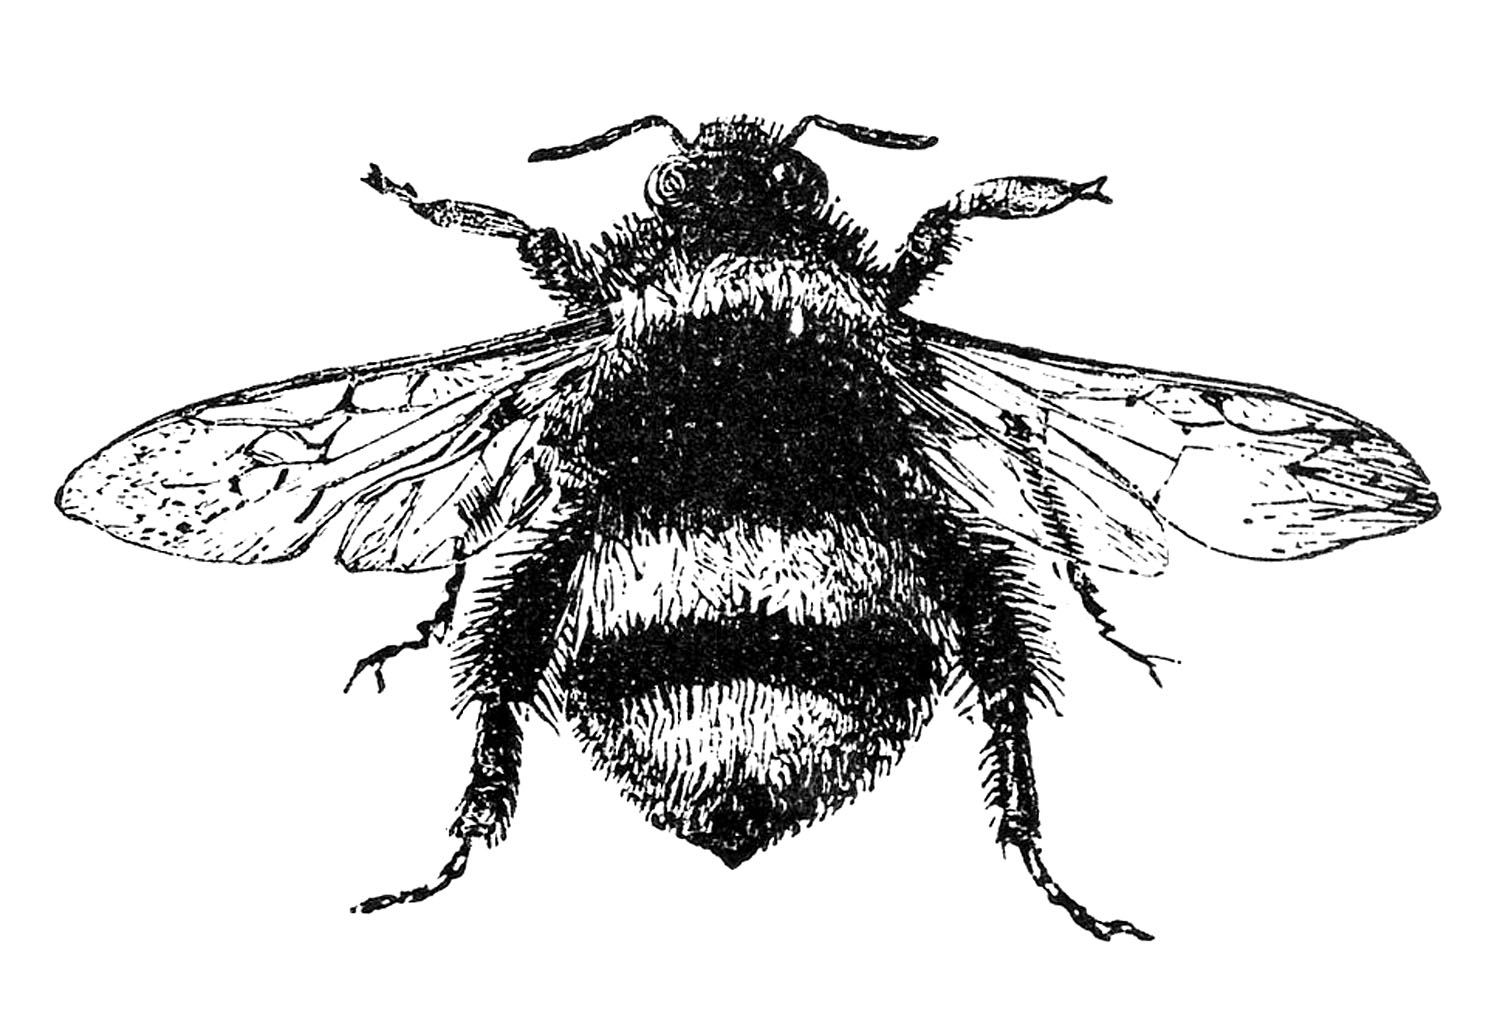
\includegraphics[scale=0.75]{img/bumblebee.jpg}
		\end{figure}
		\vspace{0.5cm}
		\Huge
		\textbf{\textsc{Metody Probabilistyczne Informatyki}}

		\vspace{0.5cm}
		\Large
		\textsc{Wybrane Dowody}

		\normalsize


		\line(1,0){330}

		\vspace{1cm}
		\textit{,,Tak teraz na to patrzę i myślę, czy ta nierówność nie powinna być w drugą stronę...''}
		\vspace{1cm}

		\textit{\textsc{Popełnione przez}}\\
		\vspace{5mm}

		\textbf{\textsc{
				Załatany Ponton \\
				V\\
				Nahtamatu\\
			}}

		\vfill

		Kraków \\
		Anno Domini 2025

	\end{center}

\end{titlepage}


\tableofcontents
\section*{Licencja}
\begin{figure}[h]
	\begin{minipage}[c]{0.25\textwidth}
		
\includegraphics[width=0.7\textwidth]{img/licencja.png}
	\end{minipage}\hfill
	\begin{minipage}[c]{0.75\textwidth}
		\caption*{
			Ten utwór jest dostępny na
			\href{https://creativecommons.org/licenses/by-sa/4.0/}{licencji Creative Commons Uznanie autorstwa
				na tych samych warunkach 4.0 Międzynarodowe.}
		}
	\end{minipage}
\end{figure}

% Remove the "Rozdział x" chapter headings, as we already number our chapters
\titleformat{\chapter}[display]{\normalfont\Huge\bfseries}{}{0pt}{\Huge}
\titlespacing*{\chapter}{0pt}{0pt}{20pt}

% Actual content
\mainmatter

\chapter{Wykład 1 (2025-10-03)}
 % Żeby nie było syfu to kolejne sekcje dodajemy do chapters/
% A potem includujemy za pomocą \input{chapters/...}

% Używamy \( \) i \[ \] zamiast dolarów -- tak jak się robi w LaTeXu


\documentclass[12pt, a4paper, polish, openany]{book}

% Please, let's familiarize ourselves with notatki.sty and tcs.sty so that we don't reinvent the wheel
\usepackage{notatki}
\fancyhead[L]{\textbf{\textit{MPI}}}

\begin{document}
% Front page and table of contents
\frontmatter

\input{titlepage}

\tableofcontents
\input{license}

% Remove the "Rozdział x" chapter headings, as we already number our chapters
\titleformat{\chapter}[display]{\normalfont\Huge\bfseries}{}{0pt}{\Huge}
\titlespacing*{\chapter}{0pt}{0pt}{20pt}

% Actual content
\mainmatter

\chapter{Wykład 1 (2025-10-03)}
\input{chapters/2025-10-03-lecture/main}

\chapter{Nagranie 1 (2025-10-04)}
\input{chapters/2025-10-04-recording/main}

\chapter{Wykład 2 (2025-10-10)}
\input{chapters/2025-10-10-lecture/main}

\chapter{Nagranie 2 (2025-10-10)}
\input{chapters/2025-10-10-recording/main}

\chapter{Wykład 3 (2025-10-17)}
\input{chapters/2025-10-17-lecture/main}

\end{document}


\chapter{Nagranie 1 (2025-10-04)}
 % Żeby nie było syfu to kolejne sekcje dodajemy do chapters/
% A potem includujemy za pomocą \input{chapters/...}

% Używamy \( \) i \[ \] zamiast dolarów -- tak jak się robi w LaTeXu


\documentclass[12pt, a4paper, polish, openany]{book}

% Please, let's familiarize ourselves with notatki.sty and tcs.sty so that we don't reinvent the wheel
\usepackage{notatki}
\fancyhead[L]{\textbf{\textit{MPI}}}

\begin{document}
% Front page and table of contents
\frontmatter

\input{titlepage}

\tableofcontents
\input{license}

% Remove the "Rozdział x" chapter headings, as we already number our chapters
\titleformat{\chapter}[display]{\normalfont\Huge\bfseries}{}{0pt}{\Huge}
\titlespacing*{\chapter}{0pt}{0pt}{20pt}

% Actual content
\mainmatter

\chapter{Wykład 1 (2025-10-03)}
\input{chapters/2025-10-03-lecture/main}

\chapter{Nagranie 1 (2025-10-04)}
\input{chapters/2025-10-04-recording/main}

\chapter{Wykład 2 (2025-10-10)}
\input{chapters/2025-10-10-lecture/main}

\chapter{Nagranie 2 (2025-10-10)}
\input{chapters/2025-10-10-recording/main}

\chapter{Wykład 3 (2025-10-17)}
\input{chapters/2025-10-17-lecture/main}

\end{document}


\chapter{Wykład 2 (2025-10-10)}
 % Żeby nie było syfu to kolejne sekcje dodajemy do chapters/
% A potem includujemy za pomocą \input{chapters/...}

% Używamy \( \) i \[ \] zamiast dolarów -- tak jak się robi w LaTeXu


\documentclass[12pt, a4paper, polish, openany]{book}

% Please, let's familiarize ourselves with notatki.sty and tcs.sty so that we don't reinvent the wheel
\usepackage{notatki}
\fancyhead[L]{\textbf{\textit{MPI}}}

\begin{document}
% Front page and table of contents
\frontmatter

\input{titlepage}

\tableofcontents
\input{license}

% Remove the "Rozdział x" chapter headings, as we already number our chapters
\titleformat{\chapter}[display]{\normalfont\Huge\bfseries}{}{0pt}{\Huge}
\titlespacing*{\chapter}{0pt}{0pt}{20pt}

% Actual content
\mainmatter

\chapter{Wykład 1 (2025-10-03)}
\input{chapters/2025-10-03-lecture/main}

\chapter{Nagranie 1 (2025-10-04)}
\input{chapters/2025-10-04-recording/main}

\chapter{Wykład 2 (2025-10-10)}
\input{chapters/2025-10-10-lecture/main}

\chapter{Nagranie 2 (2025-10-10)}
\input{chapters/2025-10-10-recording/main}

\chapter{Wykład 3 (2025-10-17)}
\input{chapters/2025-10-17-lecture/main}

\end{document}


\chapter{Nagranie 2 (2025-10-10)}
 % Żeby nie było syfu to kolejne sekcje dodajemy do chapters/
% A potem includujemy za pomocą \input{chapters/...}

% Używamy \( \) i \[ \] zamiast dolarów -- tak jak się robi w LaTeXu


\documentclass[12pt, a4paper, polish, openany]{book}

% Please, let's familiarize ourselves with notatki.sty and tcs.sty so that we don't reinvent the wheel
\usepackage{notatki}
\fancyhead[L]{\textbf{\textit{MPI}}}

\begin{document}
% Front page and table of contents
\frontmatter

\input{titlepage}

\tableofcontents
\input{license}

% Remove the "Rozdział x" chapter headings, as we already number our chapters
\titleformat{\chapter}[display]{\normalfont\Huge\bfseries}{}{0pt}{\Huge}
\titlespacing*{\chapter}{0pt}{0pt}{20pt}

% Actual content
\mainmatter

\chapter{Wykład 1 (2025-10-03)}
\input{chapters/2025-10-03-lecture/main}

\chapter{Nagranie 1 (2025-10-04)}
\input{chapters/2025-10-04-recording/main}

\chapter{Wykład 2 (2025-10-10)}
\input{chapters/2025-10-10-lecture/main}

\chapter{Nagranie 2 (2025-10-10)}
\input{chapters/2025-10-10-recording/main}

\chapter{Wykład 3 (2025-10-17)}
\input{chapters/2025-10-17-lecture/main}

\end{document}


\chapter{Wykład 3 (2025-10-17)}
 % Żeby nie było syfu to kolejne sekcje dodajemy do chapters/
% A potem includujemy za pomocą \input{chapters/...}

% Używamy \( \) i \[ \] zamiast dolarów -- tak jak się robi w LaTeXu


\documentclass[12pt, a4paper, polish, openany]{book}

% Please, let's familiarize ourselves with notatki.sty and tcs.sty so that we don't reinvent the wheel
\usepackage{notatki}
\fancyhead[L]{\textbf{\textit{MPI}}}

\begin{document}
% Front page and table of contents
\frontmatter

\input{titlepage}

\tableofcontents
\input{license}

% Remove the "Rozdział x" chapter headings, as we already number our chapters
\titleformat{\chapter}[display]{\normalfont\Huge\bfseries}{}{0pt}{\Huge}
\titlespacing*{\chapter}{0pt}{0pt}{20pt}

% Actual content
\mainmatter

\chapter{Wykład 1 (2025-10-03)}
\input{chapters/2025-10-03-lecture/main}

\chapter{Nagranie 1 (2025-10-04)}
\input{chapters/2025-10-04-recording/main}

\chapter{Wykład 2 (2025-10-10)}
\input{chapters/2025-10-10-lecture/main}

\chapter{Nagranie 2 (2025-10-10)}
\input{chapters/2025-10-10-recording/main}

\chapter{Wykład 3 (2025-10-17)}
\input{chapters/2025-10-17-lecture/main}

\end{document}


\end{document}


\chapter{Wykład 3 (2025-10-17)}
 % Żeby nie było syfu to kolejne sekcje dodajemy do chapters/
% A potem includujemy za pomocą \input{chapters/...}

% Używamy \( \) i \[ \] zamiast dolarów -- tak jak się robi w LaTeXu


\documentclass[12pt, a4paper, polish, openany]{book}

% Please, let's familiarize ourselves with notatki.sty and tcs.sty so that we don't reinvent the wheel
\usepackage{notatki}
\fancyhead[L]{\textbf{\textit{MPI}}}

\begin{document}
% Front page and table of contents
\frontmatter

\begin{titlepage}

	\begin{center}
		\begin{figure}[h]
			\centering
			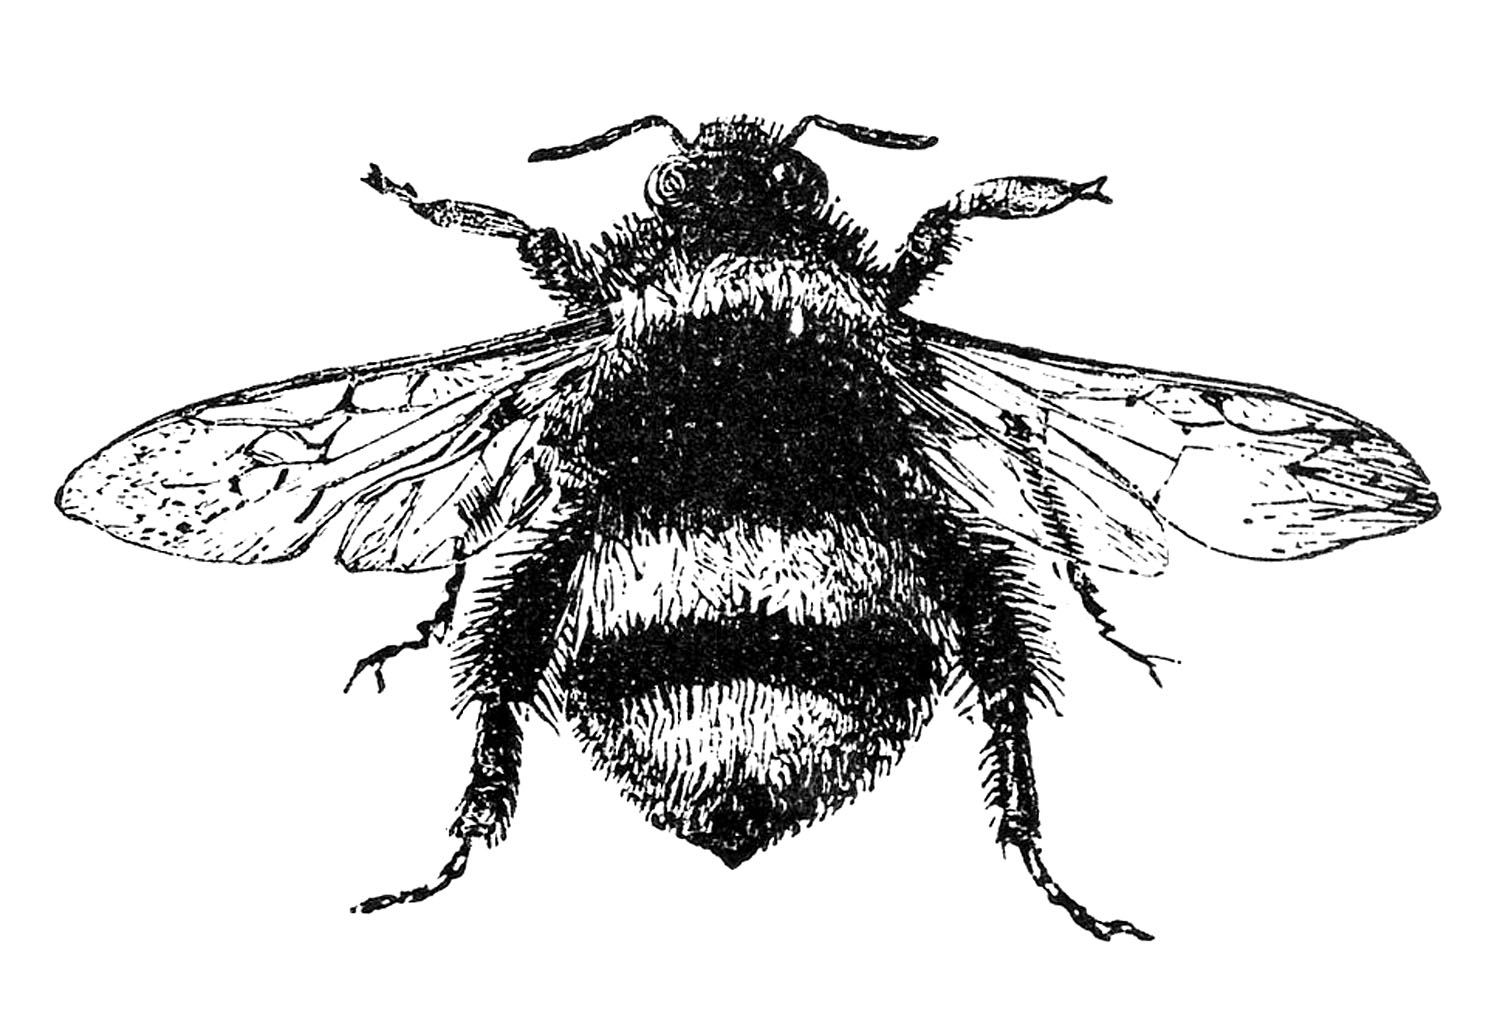
\includegraphics[scale=0.75]{img/bumblebee.jpg}
		\end{figure}
		\vspace{0.5cm}
		\Huge
		\textbf{\textsc{Metody Probabilistyczne Informatyki}}

		\vspace{0.5cm}
		\Large
		\textsc{Wybrane Dowody}

		\normalsize


		\line(1,0){330}

		\vspace{1cm}
		\textit{,,Tak teraz na to patrzę i myślę, czy ta nierówność nie powinna być w drugą stronę...''}
		\vspace{1cm}

		\textit{\textsc{Popełnione przez}}\\
		\vspace{5mm}

		\textbf{\textsc{
				Załatany Ponton \\
				V\\
				Nahtamatu\\
			}}

		\vfill

		Kraków \\
		Anno Domini 2025

	\end{center}

\end{titlepage}


\tableofcontents
\section*{Licencja}
\begin{figure}[h]
	\begin{minipage}[c]{0.25\textwidth}
		
\includegraphics[width=0.7\textwidth]{img/licencja.png}
	\end{minipage}\hfill
	\begin{minipage}[c]{0.75\textwidth}
		\caption*{
			Ten utwór jest dostępny na
			\href{https://creativecommons.org/licenses/by-sa/4.0/}{licencji Creative Commons Uznanie autorstwa
				na tych samych warunkach 4.0 Międzynarodowe.}
		}
	\end{minipage}
\end{figure}

% Remove the "Rozdział x" chapter headings, as we already number our chapters
\titleformat{\chapter}[display]{\normalfont\Huge\bfseries}{}{0pt}{\Huge}
\titlespacing*{\chapter}{0pt}{0pt}{20pt}

% Actual content
\mainmatter

\chapter{Wykład 1 (2025-10-03)}
 % Żeby nie było syfu to kolejne sekcje dodajemy do chapters/
% A potem includujemy za pomocą \input{chapters/...}

% Używamy \( \) i \[ \] zamiast dolarów -- tak jak się robi w LaTeXu


\documentclass[12pt, a4paper, polish, openany]{book}

% Please, let's familiarize ourselves with notatki.sty and tcs.sty so that we don't reinvent the wheel
\usepackage{notatki}
\fancyhead[L]{\textbf{\textit{MPI}}}

\begin{document}
% Front page and table of contents
\frontmatter

\input{titlepage}

\tableofcontents
\input{license}

% Remove the "Rozdział x" chapter headings, as we already number our chapters
\titleformat{\chapter}[display]{\normalfont\Huge\bfseries}{}{0pt}{\Huge}
\titlespacing*{\chapter}{0pt}{0pt}{20pt}

% Actual content
\mainmatter

\chapter{Wykład 1 (2025-10-03)}
\input{chapters/2025-10-03-lecture/main}

\chapter{Nagranie 1 (2025-10-04)}
\input{chapters/2025-10-04-recording/main}

\chapter{Wykład 2 (2025-10-10)}
\input{chapters/2025-10-10-lecture/main}

\chapter{Nagranie 2 (2025-10-10)}
\input{chapters/2025-10-10-recording/main}

\chapter{Wykład 3 (2025-10-17)}
\input{chapters/2025-10-17-lecture/main}

\end{document}


\chapter{Nagranie 1 (2025-10-04)}
 % Żeby nie było syfu to kolejne sekcje dodajemy do chapters/
% A potem includujemy za pomocą \input{chapters/...}

% Używamy \( \) i \[ \] zamiast dolarów -- tak jak się robi w LaTeXu


\documentclass[12pt, a4paper, polish, openany]{book}

% Please, let's familiarize ourselves with notatki.sty and tcs.sty so that we don't reinvent the wheel
\usepackage{notatki}
\fancyhead[L]{\textbf{\textit{MPI}}}

\begin{document}
% Front page and table of contents
\frontmatter

\input{titlepage}

\tableofcontents
\input{license}

% Remove the "Rozdział x" chapter headings, as we already number our chapters
\titleformat{\chapter}[display]{\normalfont\Huge\bfseries}{}{0pt}{\Huge}
\titlespacing*{\chapter}{0pt}{0pt}{20pt}

% Actual content
\mainmatter

\chapter{Wykład 1 (2025-10-03)}
\input{chapters/2025-10-03-lecture/main}

\chapter{Nagranie 1 (2025-10-04)}
\input{chapters/2025-10-04-recording/main}

\chapter{Wykład 2 (2025-10-10)}
\input{chapters/2025-10-10-lecture/main}

\chapter{Nagranie 2 (2025-10-10)}
\input{chapters/2025-10-10-recording/main}

\chapter{Wykład 3 (2025-10-17)}
\input{chapters/2025-10-17-lecture/main}

\end{document}


\chapter{Wykład 2 (2025-10-10)}
 % Żeby nie było syfu to kolejne sekcje dodajemy do chapters/
% A potem includujemy za pomocą \input{chapters/...}

% Używamy \( \) i \[ \] zamiast dolarów -- tak jak się robi w LaTeXu


\documentclass[12pt, a4paper, polish, openany]{book}

% Please, let's familiarize ourselves with notatki.sty and tcs.sty so that we don't reinvent the wheel
\usepackage{notatki}
\fancyhead[L]{\textbf{\textit{MPI}}}

\begin{document}
% Front page and table of contents
\frontmatter

\input{titlepage}

\tableofcontents
\input{license}

% Remove the "Rozdział x" chapter headings, as we already number our chapters
\titleformat{\chapter}[display]{\normalfont\Huge\bfseries}{}{0pt}{\Huge}
\titlespacing*{\chapter}{0pt}{0pt}{20pt}

% Actual content
\mainmatter

\chapter{Wykład 1 (2025-10-03)}
\input{chapters/2025-10-03-lecture/main}

\chapter{Nagranie 1 (2025-10-04)}
\input{chapters/2025-10-04-recording/main}

\chapter{Wykład 2 (2025-10-10)}
\input{chapters/2025-10-10-lecture/main}

\chapter{Nagranie 2 (2025-10-10)}
\input{chapters/2025-10-10-recording/main}

\chapter{Wykład 3 (2025-10-17)}
\input{chapters/2025-10-17-lecture/main}

\end{document}


\chapter{Nagranie 2 (2025-10-10)}
 % Żeby nie było syfu to kolejne sekcje dodajemy do chapters/
% A potem includujemy za pomocą \input{chapters/...}

% Używamy \( \) i \[ \] zamiast dolarów -- tak jak się robi w LaTeXu


\documentclass[12pt, a4paper, polish, openany]{book}

% Please, let's familiarize ourselves with notatki.sty and tcs.sty so that we don't reinvent the wheel
\usepackage{notatki}
\fancyhead[L]{\textbf{\textit{MPI}}}

\begin{document}
% Front page and table of contents
\frontmatter

\input{titlepage}

\tableofcontents
\input{license}

% Remove the "Rozdział x" chapter headings, as we already number our chapters
\titleformat{\chapter}[display]{\normalfont\Huge\bfseries}{}{0pt}{\Huge}
\titlespacing*{\chapter}{0pt}{0pt}{20pt}

% Actual content
\mainmatter

\chapter{Wykład 1 (2025-10-03)}
\input{chapters/2025-10-03-lecture/main}

\chapter{Nagranie 1 (2025-10-04)}
\input{chapters/2025-10-04-recording/main}

\chapter{Wykład 2 (2025-10-10)}
\input{chapters/2025-10-10-lecture/main}

\chapter{Nagranie 2 (2025-10-10)}
\input{chapters/2025-10-10-recording/main}

\chapter{Wykład 3 (2025-10-17)}
\input{chapters/2025-10-17-lecture/main}

\end{document}


\chapter{Wykład 3 (2025-10-17)}
 % Żeby nie było syfu to kolejne sekcje dodajemy do chapters/
% A potem includujemy za pomocą \input{chapters/...}

% Używamy \( \) i \[ \] zamiast dolarów -- tak jak się robi w LaTeXu


\documentclass[12pt, a4paper, polish, openany]{book}

% Please, let's familiarize ourselves with notatki.sty and tcs.sty so that we don't reinvent the wheel
\usepackage{notatki}
\fancyhead[L]{\textbf{\textit{MPI}}}

\begin{document}
% Front page and table of contents
\frontmatter

\input{titlepage}

\tableofcontents
\input{license}

% Remove the "Rozdział x" chapter headings, as we already number our chapters
\titleformat{\chapter}[display]{\normalfont\Huge\bfseries}{}{0pt}{\Huge}
\titlespacing*{\chapter}{0pt}{0pt}{20pt}

% Actual content
\mainmatter

\chapter{Wykład 1 (2025-10-03)}
\input{chapters/2025-10-03-lecture/main}

\chapter{Nagranie 1 (2025-10-04)}
\input{chapters/2025-10-04-recording/main}

\chapter{Wykład 2 (2025-10-10)}
\input{chapters/2025-10-10-lecture/main}

\chapter{Nagranie 2 (2025-10-10)}
\input{chapters/2025-10-10-recording/main}

\chapter{Wykład 3 (2025-10-17)}
\input{chapters/2025-10-17-lecture/main}

\end{document}


\end{document}


\end{document}



\end{document}